% Options for packages loaded elsewhere
\PassOptionsToPackage{unicode}{hyperref}
\PassOptionsToPackage{hyphens}{url}
%
\documentclass[
]{book}
\usepackage{amsmath,amssymb}
\usepackage{lmodern}
\usepackage{ifxetex,ifluatex}
\ifnum 0\ifxetex 1\fi\ifluatex 1\fi=0 % if pdftex
  \usepackage[T1]{fontenc}
  \usepackage[utf8]{inputenc}
  \usepackage{textcomp} % provide euro and other symbols
\else % if luatex or xetex
  \usepackage{unicode-math}
  \defaultfontfeatures{Scale=MatchLowercase}
  \defaultfontfeatures[\rmfamily]{Ligatures=TeX,Scale=1}
\fi
% Use upquote if available, for straight quotes in verbatim environments
\IfFileExists{upquote.sty}{\usepackage{upquote}}{}
\IfFileExists{microtype.sty}{% use microtype if available
  \usepackage[]{microtype}
  \UseMicrotypeSet[protrusion]{basicmath} % disable protrusion for tt fonts
}{}
\makeatletter
\@ifundefined{KOMAClassName}{% if non-KOMA class
  \IfFileExists{parskip.sty}{%
    \usepackage{parskip}
  }{% else
    \setlength{\parindent}{0pt}
    \setlength{\parskip}{6pt plus 2pt minus 1pt}}
}{% if KOMA class
  \KOMAoptions{parskip=half}}
\makeatother
\usepackage{xcolor}
\IfFileExists{xurl.sty}{\usepackage{xurl}}{} % add URL line breaks if available
\IfFileExists{bookmark.sty}{\usepackage{bookmark}}{\usepackage{hyperref}}
\hypersetup{
  pdftitle={Mappeeksamen},
  pdfauthor={Hermann Moen},
  hidelinks,
  pdfcreator={LaTeX via pandoc}}
\urlstyle{same} % disable monospaced font for URLs
\usepackage{longtable,booktabs,array}
\usepackage{calc} % for calculating minipage widths
% Correct order of tables after \paragraph or \subparagraph
\usepackage{etoolbox}
\makeatletter
\patchcmd\longtable{\par}{\if@noskipsec\mbox{}\fi\par}{}{}
\makeatother
% Allow footnotes in longtable head/foot
\IfFileExists{footnotehyper.sty}{\usepackage{footnotehyper}}{\usepackage{footnote}}
\makesavenoteenv{longtable}
\usepackage{graphicx}
\makeatletter
\def\maxwidth{\ifdim\Gin@nat@width>\linewidth\linewidth\else\Gin@nat@width\fi}
\def\maxheight{\ifdim\Gin@nat@height>\textheight\textheight\else\Gin@nat@height\fi}
\makeatother
% Scale images if necessary, so that they will not overflow the page
% margins by default, and it is still possible to overwrite the defaults
% using explicit options in \includegraphics[width, height, ...]{}
\setkeys{Gin}{width=\maxwidth,height=\maxheight,keepaspectratio}
% Set default figure placement to htbp
\makeatletter
\def\fps@figure{htbp}
\makeatother
\setlength{\emergencystretch}{3em} % prevent overfull lines
\providecommand{\tightlist}{%
  \setlength{\itemsep}{0pt}\setlength{\parskip}{0pt}}
\setcounter{secnumdepth}{5}
\usepackage{booktabs}
\usepackage{fontspec}
\usepackage{multirow}
\usepackage{multicol}
\usepackage{colortbl}
\usepackage{hhline}
\usepackage{longtable}
\usepackage{array}
\usepackage{hyperref}
\ifluatex
  \usepackage{selnolig}  % disable illegal ligatures
\fi
\usepackage[]{natbib}
\bibliographystyle{plainnat}

\title{Mappeeksamen}
\author{Hermann Moen}
\date{2021-12-01}

\begin{document}
\maketitle

{
\setcounter{tocdepth}{1}
\tableofcontents
}
\hypertarget{reliabilitet}{%
\chapter{Reliabilitet}\label{reliabilitet}}

\hypertarget{introduksjon}{%
\section{Introduksjon}\label{introduksjon}}

Maksimalt oksygenopptak VO2max ble først beskrevet av Hill og Lupton i 1923, og kan defineres som kroppens evne til å ta opp og forbruke oksygen per tidsenhet \citep{bassett2000, hill1923}. Innen toppidrett måles ofte det maksimale oksygenopptaket for å måle utøverens kapasitet opp mot arbeidskravet i den spesifikke idretten, og VO2max kan i så måte også sees på som et mål på den aerobe effekten til utøveren \citep{bassett2000}. I Olympiatoppens testprotokoller benytter de flere definerte hjelpekriterier for å sikre at man faktisk har funnet deltakerens maksimale oksygenopptak \citep{tønnessen2017}. Følgende kriterier er beskrevet; platå i O2 er oppnådd, økning i ventilasjon med utflating av O2 verdi, RER-verdi over 1.10 (1.05 om gjennomført laktatprofiltest i forkant) og blodlaktat over 8 \citep{tønnessen2017}.

\hypertarget{metode}{%
\section{Metode}\label{metode}}

I forkant av testen målte alle deltakerne kroppsvekten i samme klær som ble brukt under testen, men ble bedt om å ta av seg skoene. Kroppsvekten som senere brukt i beregningen av maksimalt oksygenopptak (ml kg\textsuperscript{-1} min\textsuperscript{-1}) er kroppsvekten målt i forkant av test, etter at 300g har blitt trukket av for å ta høyde for vekten av klærne. For å sikre intern validitet ble deltakerne bedt om å avstå fra anstrengende fysisk aktivitet dagen før test, standardisere måltidet i forkant av test samt avstå fra inntak av koffein under de siste 12 timene før testen \citep{halperin2015} . Pre- og post-tester ble gjennomført på samme tid på døgnet under standardiserte forhold.. Post-test ble gjennomført 6 dager etter gjennomført pretest. Det ble ikke kontrollert for fysisk aktivitet mellom testdagene.

Alle deltakerne gjennomførte en 10 minutter lang oppvarmingsprotokoll på tredemøllen (Woodway 4Front, Waukesha, USA), beskrevet for deltakerne i forkant av testen. Denne oppvarmingsprotokollen bestod av fem minutter på 11-13 i Borg 6-20 RPE skala \citep{borg1982}, etterfulgt av 2x1min på starthastighet og stigning med 30 sekund mellom. Siste tre min var også 11-13 i borg. Etter oppvarming var det to min pause før testen begynte. Starthastighet for begge kjønn var satt til 8km/t, med stigning på 10.5\% og 5.5\% for henholdsvis menn og kvinner.

VO2max ble målt ved hjelp av en metabolsk analysator med miksekammer (vyntus CPX, mixing­chamber (Vyntus CPX, Jaeger-CareFusion, UK)). Forut for alle tester ble analysatoren gass og volumkalibrert med en feillmargin på henholdsvis 2\% og 0.2\%. Analysatoren ble stilt inn til å gjøre målinger hvert 30sek, og VO2max ble kalkulert gjennom å bruke snittet av de to høyeste påfølgende målingene av O2. Underveis i testen mottok alle deltakerne en høylytt verbal oppmuntring fra testleder. Alle deltakerne gjennomførte også begge testene med samme testleder og med samme personer til stede i rommet for å redusere konfundering \citep{halperin2015}.

For hvert medgåtte minutt av testen ble hastigheten på møllen økt med 1km/t, helt til utmattelse, hvor testen ble avsluttet. Deltakernes hjertefrekvens ble også registrert under hele testen. Når testen ble avsluttet ble deltakerne bedt om å rapportere opplevd anstrengelse ved hjelp av Borg-skala \citep{borg1982}. Maksimal hjertefrekvens under testen ble også registrert. Ett minutt etter avsluttet test ble hjertefrekvens registrert, og det ble målt og analysert blodlaktat (Biosen C-line, EKF Diagnostics, Barleben, Germany).

\hypertarget{resultater}{%
\section{Resultater}\label{resultater}}

\providecommand{\docline}[3]{\noalign{\global\setlength{\arrayrulewidth}{#1}}\arrayrulecolor[HTML]{#2}\cline{#3}}

\setlength{\tabcolsep}{2pt}

\renewcommand*{\arraystretch}{1.5}

\begin{longtable}[c]{|p{1.08in}|p{1.02in}|p{1.02in}}



\hhline{>{\arrayrulecolor[HTML]{666666}\global\arrayrulewidth=2pt}->{\arrayrulecolor[HTML]{666666}\global\arrayrulewidth=2pt}->{\arrayrulecolor[HTML]{666666}\global\arrayrulewidth=2pt}-}

\multicolumn{1}{!{\color[HTML]{000000}\vrule width 0pt}>{\raggedright}p{\dimexpr 1.08in+0\tabcolsep+0\arrayrulewidth}}{\fontsize{11}{11}\selectfont{\textcolor[HTML]{000000}{\global\setmainfont{Arial}{}}}} & \multicolumn{1}{!{\color[HTML]{000000}\vrule width 0pt}>{\raggedright}p{\dimexpr 1.02in+0\tabcolsep+0\arrayrulewidth}}{\fontsize{11}{11}\selectfont{\textcolor[HTML]{000000}{\global\setmainfont{Arial}{Kvinner}}}} & \multicolumn{1}{!{\color[HTML]{000000}\vrule width 0pt}>{\raggedright}p{\dimexpr 1.02in+0\tabcolsep+0\arrayrulewidth}!{\color[HTML]{000000}\vrule width 0pt}}{\fontsize{11}{11}\selectfont{\textcolor[HTML]{000000}{\global\setmainfont{Arial}{Menn}}}} \\

\hhline{>{\arrayrulecolor[HTML]{666666}\global\arrayrulewidth=2pt}->{\arrayrulecolor[HTML]{666666}\global\arrayrulewidth=2pt}->{\arrayrulecolor[HTML]{666666}\global\arrayrulewidth=2pt}-}

\endfirsthead

\hhline{>{\arrayrulecolor[HTML]{666666}\global\arrayrulewidth=2pt}->{\arrayrulecolor[HTML]{666666}\global\arrayrulewidth=2pt}->{\arrayrulecolor[HTML]{666666}\global\arrayrulewidth=2pt}-}

\multicolumn{1}{!{\color[HTML]{000000}\vrule width 0pt}>{\raggedright}p{\dimexpr 1.08in+0\tabcolsep+0\arrayrulewidth}}{\fontsize{11}{11}\selectfont{\textcolor[HTML]{000000}{\global\setmainfont{Arial}{}}}} & \multicolumn{1}{!{\color[HTML]{000000}\vrule width 0pt}>{\raggedright}p{\dimexpr 1.02in+0\tabcolsep+0\arrayrulewidth}}{\fontsize{11}{11}\selectfont{\textcolor[HTML]{000000}{\global\setmainfont{Arial}{Kvinner}}}} & \multicolumn{1}{!{\color[HTML]{000000}\vrule width 0pt}>{\raggedright}p{\dimexpr 1.02in+0\tabcolsep+0\arrayrulewidth}!{\color[HTML]{000000}\vrule width 0pt}}{\fontsize{11}{11}\selectfont{\textcolor[HTML]{000000}{\global\setmainfont{Arial}{Menn}}}} \\

\hhline{>{\arrayrulecolor[HTML]{666666}\global\arrayrulewidth=2pt}->{\arrayrulecolor[HTML]{666666}\global\arrayrulewidth=2pt}->{\arrayrulecolor[HTML]{666666}\global\arrayrulewidth=2pt}-}\endhead



\multicolumn{3}{!{\color[HTML]{FFFFFF}\vrule width 0pt}>{\raggedright}p{\dimexpr 3.13in+4\tabcolsep+2\arrayrulewidth}!{\color[HTML]{FFFFFF}\vrule width 0pt}}{\fontsize{11}{11}\selectfont{\textcolor[HTML]{000000}{\global\setmainfont{Arial}{Verdier\ er\ gitt\ som\ gjennomsnitt\ og\ (Standardavvik)}}}} \\

\endfoot



\multicolumn{1}{!{\color[HTML]{000000}\vrule width 0pt}>{\raggedright}p{\dimexpr 1.08in+0\tabcolsep+0\arrayrulewidth}}{\fontsize{11}{11}\selectfont{\textcolor[HTML]{000000}{\global\setmainfont{Arial}{N}}}} & \multicolumn{1}{!{\color[HTML]{000000}\vrule width 0pt}>{\raggedright}p{\dimexpr 1.02in+0\tabcolsep+0\arrayrulewidth}}{\fontsize{11}{11}\selectfont{\textcolor[HTML]{000000}{\global\setmainfont{Arial}{4}}}} & \multicolumn{1}{!{\color[HTML]{000000}\vrule width 0pt}>{\raggedright}p{\dimexpr 1.02in+0\tabcolsep+0\arrayrulewidth}!{\color[HTML]{000000}\vrule width 0pt}}{\fontsize{11}{11}\selectfont{\textcolor[HTML]{000000}{\global\setmainfont{Arial}{7}}}} \\





\multicolumn{1}{!{\color[HTML]{000000}\vrule width 0pt}>{\raggedright}p{\dimexpr 1.08in+0\tabcolsep+0\arrayrulewidth}}{\fontsize{11}{11}\selectfont{\textcolor[HTML]{000000}{\global\setmainfont{Arial}{Alder\ (år)}}}} & \multicolumn{1}{!{\color[HTML]{000000}\vrule width 0pt}>{\raggedright}p{\dimexpr 1.02in+0\tabcolsep+0\arrayrulewidth}}{\fontsize{11}{11}\selectfont{\textcolor[HTML]{000000}{\global\setmainfont{Arial}{24.5\ (1.29)}}}} & \multicolumn{1}{!{\color[HTML]{000000}\vrule width 0pt}>{\raggedright}p{\dimexpr 1.02in+0\tabcolsep+0\arrayrulewidth}!{\color[HTML]{000000}\vrule width 0pt}}{\fontsize{11}{11}\selectfont{\textcolor[HTML]{000000}{\global\setmainfont{Arial}{23.9\ (1.77)}}}} \\





\multicolumn{1}{!{\color[HTML]{000000}\vrule width 0pt}>{\raggedright}p{\dimexpr 1.08in+0\tabcolsep+0\arrayrulewidth}}{\fontsize{11}{11}\selectfont{\textcolor[HTML]{000000}{\global\setmainfont{Arial}{Vekt\ (kg)}}}} & \multicolumn{1}{!{\color[HTML]{000000}\vrule width 0pt}>{\raggedright}p{\dimexpr 1.02in+0\tabcolsep+0\arrayrulewidth}}{\fontsize{11}{11}\selectfont{\textcolor[HTML]{000000}{\global\setmainfont{Arial}{58.9\ (6.28)}}}} & \multicolumn{1}{!{\color[HTML]{000000}\vrule width 0pt}>{\raggedright}p{\dimexpr 1.02in+0\tabcolsep+0\arrayrulewidth}!{\color[HTML]{000000}\vrule width 0pt}}{\fontsize{11}{11}\selectfont{\textcolor[HTML]{000000}{\global\setmainfont{Arial}{74.8\ (5.55)}}}} \\





\multicolumn{1}{!{\color[HTML]{000000}\vrule width 0pt}>{\raggedright}p{\dimexpr 1.08in+0\tabcolsep+0\arrayrulewidth}}{\fontsize{11}{11}\selectfont{\textcolor[HTML]{000000}{\global\setmainfont{Arial}{Høyde\ (cm)}}}} & \multicolumn{1}{!{\color[HTML]{000000}\vrule width 0pt}>{\raggedright}p{\dimexpr 1.02in+0\tabcolsep+0\arrayrulewidth}}{\fontsize{11}{11}\selectfont{\textcolor[HTML]{000000}{\global\setmainfont{Arial}{166\ (2.99)}}}} & \multicolumn{1}{!{\color[HTML]{000000}\vrule width 0pt}>{\raggedright}p{\dimexpr 1.02in+0\tabcolsep+0\arrayrulewidth}!{\color[HTML]{000000}\vrule width 0pt}}{\fontsize{11}{11}\selectfont{\textcolor[HTML]{000000}{\global\setmainfont{Arial}{180\ (3.1)}}}} \\

\hhline{>{\arrayrulecolor[HTML]{666666}\global\arrayrulewidth=2pt}->{\arrayrulecolor[HTML]{666666}\global\arrayrulewidth=2pt}->{\arrayrulecolor[HTML]{666666}\global\arrayrulewidth=2pt}-}



\end{longtable}

Det var 11 deltakere i studien, samtlige deltakere er studenter ved Høgskolen i Innlandet. Deskriptive data for disse deltakerne er vist i Tabell 1, i Figur 1 kan man se utviklingen fra pre-test til post-test fordelt på kjønn. Det typiske målefeilet (typical error, \citep{hopkins2000}) fra pre til post-test er utregnet til å være 4.04\%.

\begin{figure}
\centering
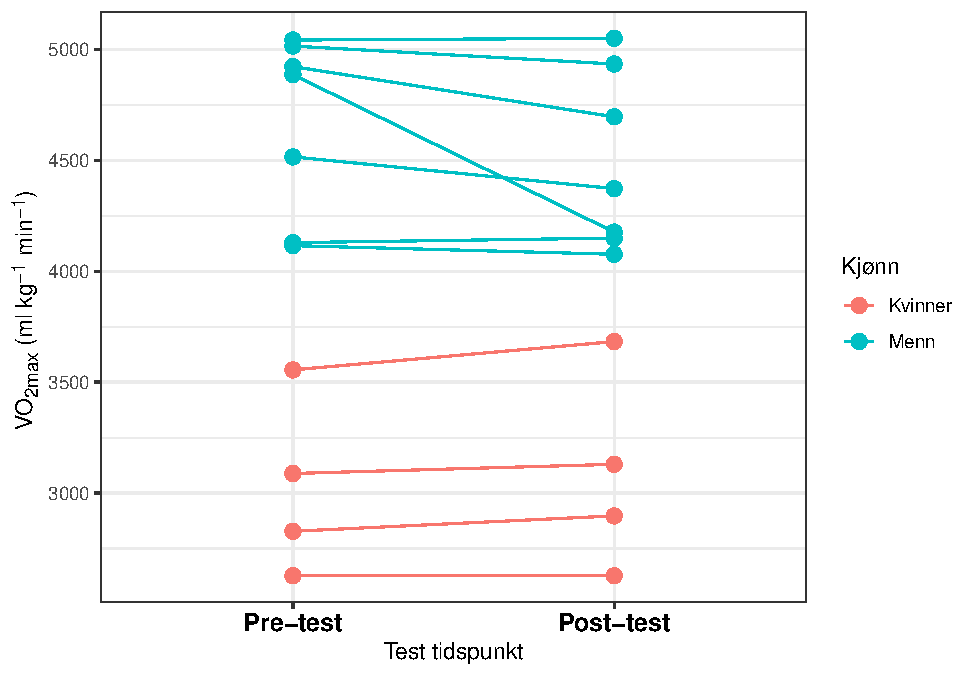
\includegraphics{_main_files/figure-latex/Figur-1.pdf}
\caption{\label{fig:Figur}Figurtekst legg til\ldots{}}
\end{figure}

\hypertarget{diskusjon}{%
\section{Diskusjon}\label{diskusjon}}

Ettersom testing av maksimalt oksygenopptak er en test som gjennomføres til utmattelse, vil man kunne forvente en viss variasjon i testresultatene ettersom opplevd anstrengelse kan påvirkes av flere ulike variabler \citep{halperin2015}. For å redusere konfundering vil flere faktorer være nyttig å ta hensyn til under slik testing. Som nevnt i metoden vil standardisering av matinntak, koffeininntak, utstyr og tidspunkt for gjennomføring av test være med på å kunne sikre intern validitet i resultatene. Eksempler er deltakernes kjennskap til testen, verbal oppmuntring og personer tilstede under testen er andre faktorer som potensielt kan bidra til konfundering. Felles for alle faktorer er at graden av påvirkning på resultatene muligens reduseres ved hjelp av en standardisert testprotokoll. Deltakerne - og testlederne, sin kjennskap til testen er en annen faktor som trolig påvirker resultatene i vårt prosjekt. I dette tilfellet fantes det enkelte deltakere som hadde gjennomført en liknende test flere ganger, og en kan da forvente en mindre grad av variasjon mellom resultatene på pre og post test, sammenlignet med de deltakerne som gjennomførte testen for første gang på pretest. Dette fordi kjennskapen og kunnskapen de tilegnet seg på pre-test, trolig spiller inn på testresultatene. Standardfeilen på 4.04\% kan også tyde på at enkelte av disse resultatene kan være utsatt for konfundering av ulik sort \citep{hopkins2000}.

Grunnen til at vi snakker om standardfeil er at når vi ønsker å måle påvirkningen av trening på en gruppe individer er det viktig å kunne si noe om hva som er endring og hva som er støy (målefeil). Desto mindre støy en test innebærer jo bedre er målingen. Målet som brukes er standardfeil. Hva som danner denne variasjonen som representeres ved typical error er multifaktorelt, men hoveddelen er som oftest biologisk \citep{hopkins2000}.

For å måle standardfeil har vi brukt within subject deviation metoden. Denne metoden påvirkes ikke av at gjennomsnittet endrer seg fra test til test \citep{hopkins2000}. Data for målinger i VO2max fra fem sertifiserte Australske laboratorier fastslo ett gjennomsnitt på 2.2\% for standardfeil \citep{halperin2015}. Data fra det Australske institutt for sport har også fastslått at en standardfeil på omtrent 2\% er riktig for både maksimal og submaksimal O2 \citep{clark2007, robertson2010, saunders2009}. Dette indikerer at med godt kalibrert utstyr og med utøvere som er godt vant med testingen vil en standardfeil på 2\% for det biologiske, og analytiske være riktig \citep{halperin2015}. Vår standardfeil på 4.04\% kan derfor tenkes å være et bilde hvordan det kan se ut med få deltakere, med ulikt utgangspunkt, men også uten skikkelig standardisering av treningshverdagen i forkant av testene. Det kan også tenkes at med et varierende nivå hos deltagerne kan enkelte oppleve en treningseffekt av test 1. Samtidig som andre kanskje ble slitne av å få en test inn i treningshverdagen.

\hypertarget{referanser}{%
\section{Referanser}\label{referanser}}

\hypertarget{lab-rapport}{%
\chapter{Lab rapport}\label{lab-rapport}}

\hypertarget{introduksjon-1}{%
\section{Introduksjon}\label{introduksjon-1}}

\hypertarget{vitenskapsteori}{%
\chapter{Vitenskapsteori}\label{vitenskapsteori}}

Placeholder

\hypertarget{falsifikasjon}{%
\section{Falsifikasjon}\label{falsifikasjon}}

\hypertarget{hd-metoden-og-abduksjon}{%
\section{HD-metoden og abduksjon}\label{hd-metoden-og-abduksjon}}

\hypertarget{replikasjonskrisen}{%
\section{Replikasjonskrisen}\label{replikasjonskrisen}}

  \bibliography{referanser.bib}

\end{document}
